\section{Minimização de $||\MATRIX{A}\VECTOR{x}-\VECTOR{b}||_{\MATRIX{C}}^2+\alpha ||\VECTOR{x}-\VECTOR{q}||_{\MATRIX{D}}^2$
}

\index{Problema inverso!Linear}
\index{Minimização do erro quadrático!Linear}


\begin{theorem}\label{theo:minAxbCAxbplusalphaxqD}
Dados,
o escalar $\alpha \in \mathbb{R}$, 
os vetores coluna $\VECTOR{x}\in \mathbb{R}^N$, 
$\VECTOR{b}\in \mathbb{R}^M$ e
$\VECTOR{q}\in \mathbb{R}^N$,  
uma matriz $\MATRIX{A} \in \mathbb{R}^{M\times N}$, 
as matrizes diagonais $\MATRIX{C} \in \mathbb{R}^{M\times M}$ e
$\MATRIX{D} \in \mathbb{R}^{N\times N}$, e 
definida a Eq. (\ref{eq:minAxbCAxb1alphaxqD}),
\begin{equation}\label{eq:minAxbCAxb1alphaxqD}
e(\VECTOR{x})  = ||\MATRIX{A}\VECTOR{x}-\VECTOR{b}||_{\MATRIX{C}}^2 +\alpha ||\VECTOR{x}-\VECTOR{q}||_{\MATRIX{D}}^2.
\end{equation}
Se desejamos ter o valor $\VECTOR{\hat{x}}$ que minimiza o escalar $e(\VECTOR{\hat{x}})$,
devemos usar\footnote{A demostração pode ser vista na Prova \ref{proof:theo:minAxbCAxbalphaxqD}.} a Eq. (\ref{eq:minAxbCAxb2alphaxqD}),
\begin{equation}\label{eq:minAxbCAxb2alphaxqD}
\VECTOR{\hat{x}}=\left[ \MATRIX{A}^{\transpose}\MATRIX{C}\MATRIX{A} +\alpha\MATRIX{D}\right]^{-1} 
\left[ \MATRIX{A}^{\transpose}\MATRIX{C} \VECTOR{b}+\alpha\MATRIX{D}\VECTOR{q}\right].
\end{equation}
Assim, o mínimo existe só sim $\MATRIX{A}^{\transpose}\MATRIX{C}\MATRIX{A} +\alpha\MATRIX{D}$ tem inversa.
\end{theorem}



%%%%%%%%%%%%%%%%%%%%%%%%%%%%%%%%%%%%%%%%%%%%%%%%%%%%%%%%%%%%%%%%%%%%%%%%%%%%%%%%
\subsection{Exemplos de minimização de 
$||\MATRIX{A}\VECTOR{x}-\VECTOR{b}||_{\MATRIX{C}}^2+\alpha ||\VECTOR{x}-\VECTOR{q}||_{\MATRIX{D}}^2$}

\begin{example}[Procurando um ponto 
$\VECTOR{\hat{x}}$ que minimize
 $||\MATRIX{A}\VECTOR{x}-\VECTOR{b}||_{\MATRIX{C}}^2+\alpha ||\VECTOR{x}-\VECTOR{q}||_{\MATRIX{D}}^2$:]
\label{ex:minAxbCAxbplusalphaxqD1}
Conhecido 
um vetor coluna $\VECTOR{x}\in \mathbb{R}^2$,
as matrizes $\MATRIX{A} \in \mathbb{R}^{3\times 2}$, $\MATRIX{C} \in \mathbb{R}^{3\times 3}$  e $\MATRIX{D} \in \mathbb{R}^{2\times 2}$,
o escalar $\alpha \in \mathbb{R}$,
e os pontos $\VECTOR{b} \in \mathbb{R}^{3}$ e $\VECTOR{q} \in \mathbb{R}^{2}$,
achar o vetor $\VECTOR{x}$ que minimize 
$||\MATRIX{A}\VECTOR{x}-\VECTOR{b}||_{\MATRIX{C}}^2+\alpha ||\VECTOR{x}-\VECTOR{q}||_{\MATRIX{D}}^2$;
sabendo que:
\begin{equation}
\VECTOR{b}=\begin{bmatrix}
1\\
1\\
1
\end{bmatrix},
\quad 
\MATRIX{A}=\begin{bmatrix}
1 & 0\\
0 & 1\\
1 & 1
\end{bmatrix},
\quad 
\MATRIX{C}=\begin{bmatrix}
1 & 0 & 0\\
0 & 1 & 0\\
0 & 0 & 1 
\end{bmatrix},
\quad \alpha=0.5,
\quad
\VECTOR{q}=\begin{bmatrix}
0\\
0
\end{bmatrix},
\quad 
\MATRIX{D}=\begin{bmatrix}
1 & 0\\
0 & 1
\end{bmatrix}.
\end{equation}

Podemos ver a resposta a este exemplo na Solução \ref{ex:minAxbCAxbplusalphaxqD:sol1}.
\end{example}


\begin{SolutionT}[Relativa ao Exemplo \ref{ex:minAxbCAxbplusalphaxqD1}:]
\label{ex:minAxbCAxbplusalphaxqD:sol1}
Com todos estes dados e usando a Eq. (\ref{eq:minAxbCAxb1alphaxqD}),
obtemos a superficie $e(\VECTOR{x})$ como mostra a Figura \ref{fig:ex:minAxbCAxb1alphaxqD:a}.
Usando a Eq. (\ref{eq:minAxbCAxb2alphaxqD}) sabemos que o ponto $\VECTOR{\hat{x}}=[0.85714\quad 0.85714]^{\transpose}$
minimiza a Eq. (\ref{eq:minAxbCAxb1alphaxqD}), com um $e(\VECTOR{\hat{x}})=0.97714$.

\begin{figure}[h!]
         \centering
         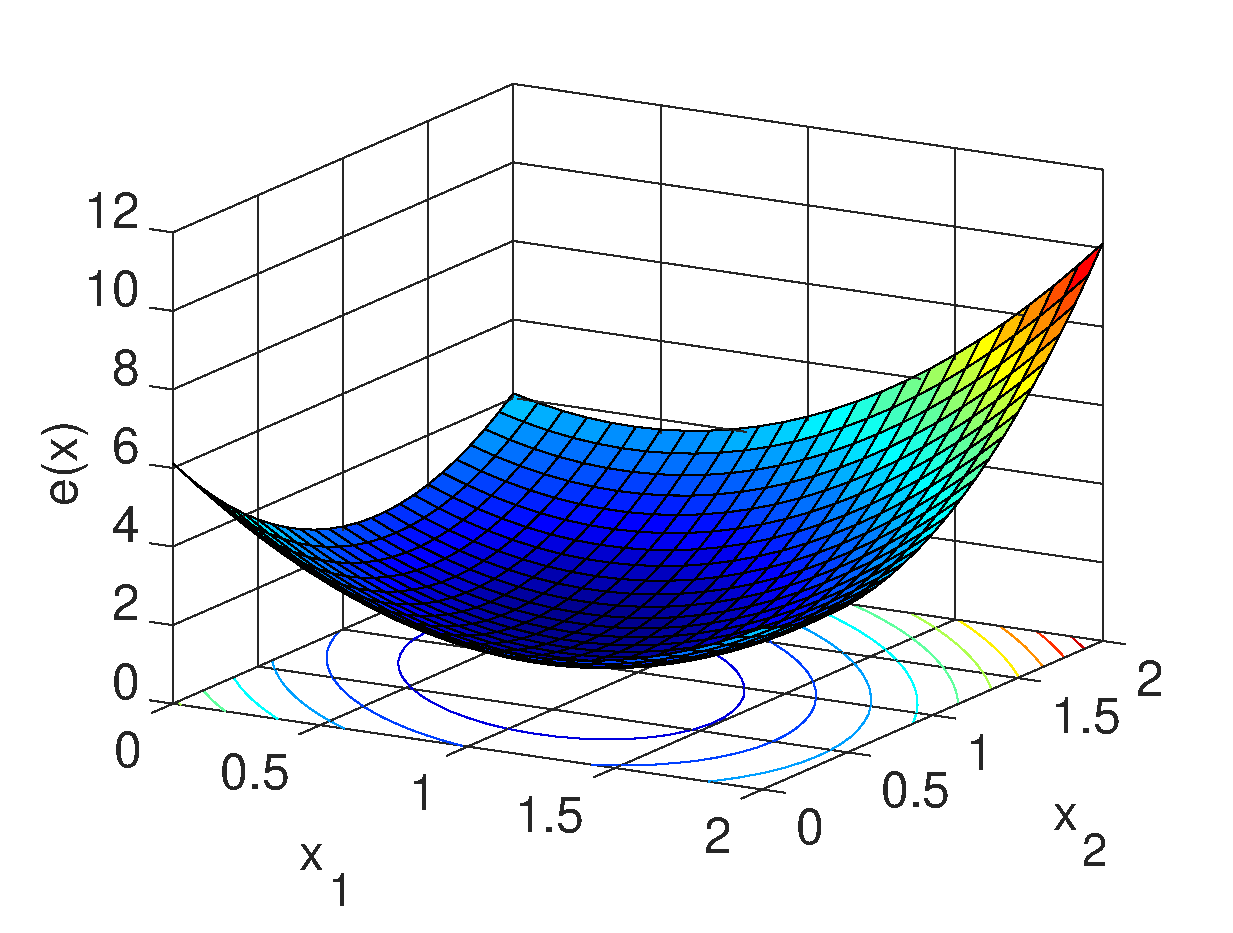
\includegraphics[width=0.6\textwidth]{chapters/minimization-fx/mfiles/axxq1/surfcex.eps}
         \caption{Superficie $e(\VECTOR{x})$. }
         \label{fig:ex:minAxbCAxb1alphaxqD:a}
\end{figure}

\end{SolutionT}

